\documentclass{article}

\usepackage[UTF8]{ctex}
\usepackage{amsmath,amssymb}
\usepackage{geometry}
\usepackage{graphicx}

\geometry{a4paper, margin=2.5cm}

\begin{document}

% ============================================================
\section*{离线强化学习：CQL 与 IQL（Offline RL）}

\subsection*{先讲一个故事}

一支球队的教练拿到了一份特殊的任务：球队已经解散，他没有办法再带队上训练场，手里只有一本过去赛季的比赛录像集。录像里记录了每一场比赛的完整过程——谁在什么局势下做了什么决定，结果如何。他要仅凭这本录像，写出一套下一场比赛的战术手册。

\textbf{朴素 RL 的做法}：把录像当作免费的训练场，反复回放、反复演练，让 Q 函数和策略在网络里「练」到收敛。

\textbf{结果出人意料}：反复演练的战术手册在录像覆盖过的场景里还行，可一旦涉及录像里从没出现过的场景，教练编出来的指令荒谬到离谱——整体水平甚至不如照着录像原样抄一遍（行为克隆）。

\textbf{本章的核心问题}：只有一份固定、不能再与真实环境交互的数据集时，如何学到不塌缩的策略？

\[
\boxed{\text{只能访问固定数据集 } \mathcal{D}=\{(s,a,r,s',d)\},\quad \text{目标是学到 } \pi \text{ 使 } \mathbb{E}_\pi\!\Big[\sum_t \gamma^t r_t\Big] \text{ 最大}}
\]

这一场病叫\textbf{分布漂移（distribution shift）}：离线学到的策略会去「询问」数据集几乎没有覆盖的状态—动作对，而网络对这些地方的回答完全失真，误差被自举逐步放大。

好消息是，这个领域有两套同样重要、同样成熟的「药方」，它们选择了截然不同的治病思路：

\textbf{CQL（方案一）}：即使必须预测没见过的动作，也\textbf{把它们的价值估计压低}——把悲观写进价值函数。

\textbf{IQL（方案二）}：\textbf{根本不去预测没见过的动作}——只在数据支持的范围内挑高价值动作，把悲观写进动作集合。

\subsection*{数学形式化}

\textbf{离线数据集}：$\mathcal{D}$ 由某个\textbf{行为策略（behavior policy）}$\mu$ 采样产生，覆盖范围由 $\mu$ 的占用分布 $d^\mu(s,a)$ 决定。数据是一次性的，$\mathcal{D}$ 不可再扩大。

\begin{itemize}
  \item $\mathcal{D}$ —— 固定数据集，训练期间只读不改；
  \item $\mu$ —— 行为策略，$\mathcal{D}$ 的「出身」，我们拿不到也不能再用它交互；
  \item $d^\mu(s,a)$ —— 行为策略的占用分布，数据只覆盖它的支撑集；
  \item $a\sim\pi(\cdot|s)$ vs $a\sim\mu(\cdot|s)$ —— 学到的策略与数据分布不匹配，这就是分布漂移的来源。
\end{itemize}

\textbf{翻译成人话}：在线 RL 里，策略每走一步都可以回到真实环境求证，错了立即纠正；离线 RL 里没有求证的机会，网络一旦问出数据之外的问题，得到的答案没有人在乎是不是真的。

% ============================================================
\section*{外推误差：朴素离线 Q-learning 为什么塌缩}

\subsection*{$\max$ 是罪魁祸首}

回忆 DQN 的目标值：
\[
y = r + \gamma \max_{a'} Q_{\bar\theta}(s', a')
\]

在线时，持续交互会不断用新数据校准 $\max$ 挑中的高估动作；离线时，$\max$ 遍历的是网络对\textbf{所有动作}（包括数据集里从未出现过的动作）的估计，且再没有新数据来修正它们。对于没见过的动作，$Q_{\bar\theta}(s',a')$ 从没有被任何目标值校准过，它的取值是网络「自由发挥」的——$\max$ 会稳定地选中「相对最高」的那个，而它往往正是数据外、不可信的那个。这个不可信的高值再作为自举目标反向放大，Q 估计与真实价值逐渐\textbf{脱钩}，贪心策略据此行动，真实回报随之崩盘（图 1）。

Fujimoto 等把其中最主要的来源——动作不存在于数据——称为\textbf{外推误差（extrapolation error）}；Levine 等（2020）的综述进一步把这类误差归纳为三类来源：

\begin{itemize}
  \item \textbf{动作不存在于数据}：$\max$ 选中的 $a'$ 在 $\mathcal{D}$ 中从未出现，Q 对它没有依据；
  \item \textbf{状态不匹配}：$s'$ 在 $\mathcal{D}$ 中罕见（或从未出现），该状态下的所有动作估计都不可信；
  \item \textbf{环境动态不匹配}：即使 $(s',a')$ 在数据里，离线假定的转移与真实环境也可能不同。
\end{itemize}

\begin{figure}[!htbp]
  \centering
  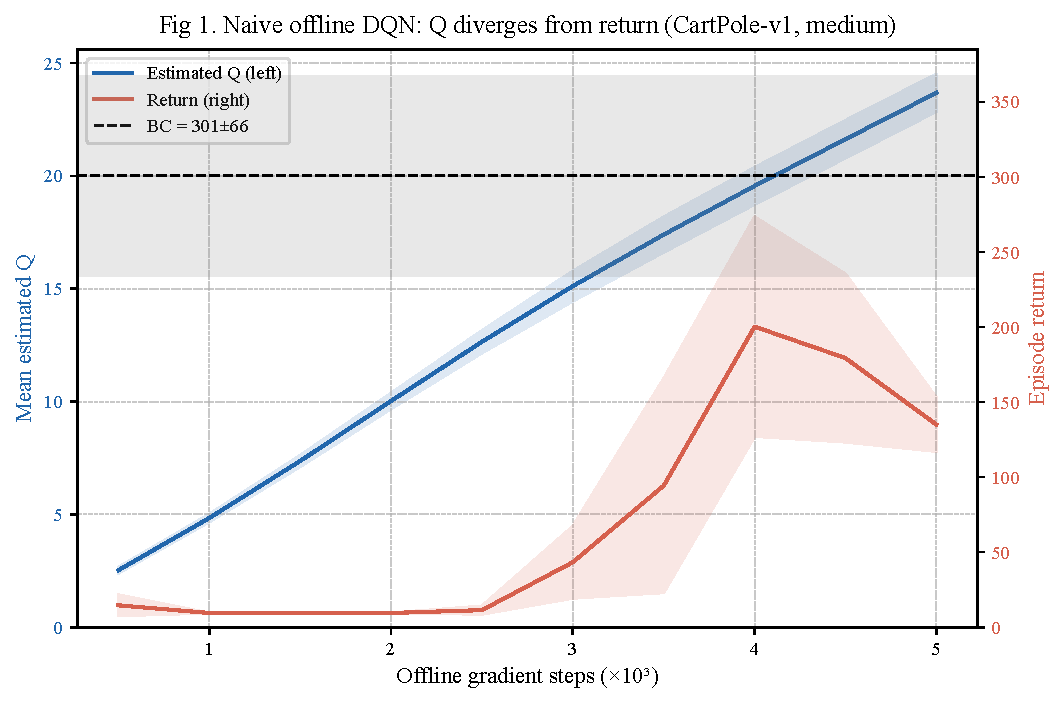
\includegraphics[width=0.88\textwidth]{fig1_ood_overestimation.pdf}
  \caption{朴素离线 DQN 的外推误差塌缩（CartPole-v1，medium 数据集，3 个随机种子，阴影为 $\pm 1\sigma$）。同一张图里：蓝色曲线（左轴）是 Q 网络对数据状态的最大 Q 估计——它不再跟踪策略的真实价值；红色曲线（右轴）是贪心策略的真实回报，短暂改善后回落，且始终远低于行为克隆（BC）这条「及格线」（BC 约 300，见图 2 的灰色区间）。Q 估计与真实回报脱钩——正是外推误差进入自举目标后的表现。}
  \label{fig:offline-overestimation}
\end{figure}

\subsection*{Q 值与真实价值的脱钩}

过估计不直接等同于「Q 数值大」。诊断离线算法不能只看 Q 的高低，而要看 \textbf{Q 估计与真实回报是否脱钩}：图 1 中朴素离线 DQN 的回报先升后跌、始终远低于 BC，而 Q 估计并不反映策略的真实价值——Q 的高低，并不代表策略好坏。一个健康的算法应该让 Q 与回报\textbf{同步}：价值兑现为回报，回报反过来印证价值。CQL 与 IQL 正是通过掐断数据外高值的来源，把回报稳定恢复到 BC 水平（图 2、图 3）。

% ============================================================
\section*{及格线：行为克隆（Behavior Cloning）}

在给出两套药方之前，先立一条参照线。

\textbf{行为克隆}把离线学习变成一个纯监督学习问题：直接拟合行为策略，
\[
\pi_\text{BC} = \arg\max_\pi \mathbb{E}_{(s,a)\sim\mathcal{D}}\!\left[\log\pi(a|s)\right]
\]

BC 的上限是\textbf{数据集本身的质量}：再好的监督拟合也复现不出数据里没有出现过的行为。注意，「数据集的质量」不等于行为策略 $\mu$ 的平均水平——本章数据由 $\mu$ 以 $\varepsilon=0.3$ 的随机性采集（$\mu$ 平均回报约 111），数据里仍有约 70\% 的状态—动作对来自贪心决策，BC 可以从中「去噪」，恢复出比 $\mu$ 平均水平更好的策略（约 300，均值）。因此 BC 的意义不在「复刻 $\mu$」，而在\textbf{给离线学习立一条不塌缩的及格线}。

BC 的下限意义是：它告诉我们\textbf{不塌缩}的最低要求。朴素离线 Q-learning 连 BC 都打不过（图 1），说明它的失败不是「学得不够好」，而是「学坏了」——方向错了。一个合格的离线算法至少要把回报恢复到 BC 的水平：

\begin{itemize}
  \item 数据质量高（expert）时，好的离线算法可以明显\textbf{超越} BC；
  \item 数据质量低（random）时，任何离线算法都\textbf{不应低于} BC。
\end{itemize}

由于 BC 本身有训练方差（本章图中用灰色区间带表示 mean $\pm 1\sigma$），「恢复到 BC 水平」比「严格超过某一个数」更稳健——这也是图 2、图 3 采用的判据。

以下两节就是达到这条及格线的两套方案。

% ============================================================
\section*{方案一：CQL——把悲观写进价值函数}

\subsection*{直觉}

保守 Q 学习（Conservative Q-Learning）保留对\textbf{所有动作}的评估，但给「数据之外的动作」加一笔\textbf{悲观惩罚}，压低它们的 Q 估计。惩罚让贪心决策自然落在数据支撑内的动作上——不是不许问，而是\textbf{问了也知道不值}。

\subsection*{保守正则化项}

对每个状态 $s$，CQL 在标准 Bellman 误差之外加一项正则。其中行为策略 $\mu$ 在离线场景下不可知，以数据集中的\textbf{经验分布} $\hat\mu(a|s)$ 估计之（即状态 $s$ 下各动作在 $\mathcal{D}$ 中的出现频率）：
\[
\boxed{\mathcal{R}(s) \;=\; \log\sum_{a}\exp Q_\theta(s,a) \;-\; \mathbb{E}_{a\sim\hat\mu(\cdot|s)}\!\left[Q_\theta(s,a)\right]}
\]

\begin{itemize}
  \item $\log\sum_a\exp Q_\theta(s,a)$（logsumexp 项）——在最小化 $L_\text{CQL}$ 时把 Q 往下压，且 softmax 权重集中在\textbf{高 Q 的动作}上，数据外的高值动作首当其冲；
  \item $-\mathbb{E}_{a\sim\hat\mu(\cdot|s)}[Q_\theta(s,a)]$——在最小化时把\textbf{数据内}动作的 Q 往上抬。
\end{itemize}

一压一抬：数据内动作的相对价值被抬高，数据外动作的相对价值被压低。整体对 $\max$ 的行为没有任何显式约束，但贪心选择的方向被惩罚项拧回了数据内。

\subsection*{完整目标}

\[
\boxed{L_\text{CQL}(\theta) = \alpha\,\mathbb{E}_{s\sim\mathcal{D}}\!\left[\mathcal{R}(s)\right] \;+\; \frac{1}{2}\,\mathbb{E}_{(s,a,s')\sim\mathcal{D}}\!\left[\bigl(Q_\theta(s,a) - \hat{\mathcal{T}}^\pi \bar Q(s,a)\bigr)^2\right]}
\]

\begin{itemize}
  \item 第二项是标准 Bellman 误差，$\hat{\mathcal{T}}^\pi$ 为基于样本的贝尔曼算子，$Q_{\bar\theta}$ 为目标网络；
  \item $\alpha > 0$ 是\textbf{保守强度}：$\alpha$ 越大，对数据外动作压得越狠（也更保守）；$\alpha \to 0$ 退化为朴素离线 Q-learning。
\end{itemize}

\textbf{为什么这样设计}：Q 与回报脱钩的正反馈来源于 $\max$ 选中的数据外动作。CQL 不堵 $\max$ 的嘴，而是让每个数据外动作的 Q 都「长得比数据内动作慢」，不可信高值的来源被掐断，脱钩随之消失。

\begin{figure}[!htbp]
  \centering
  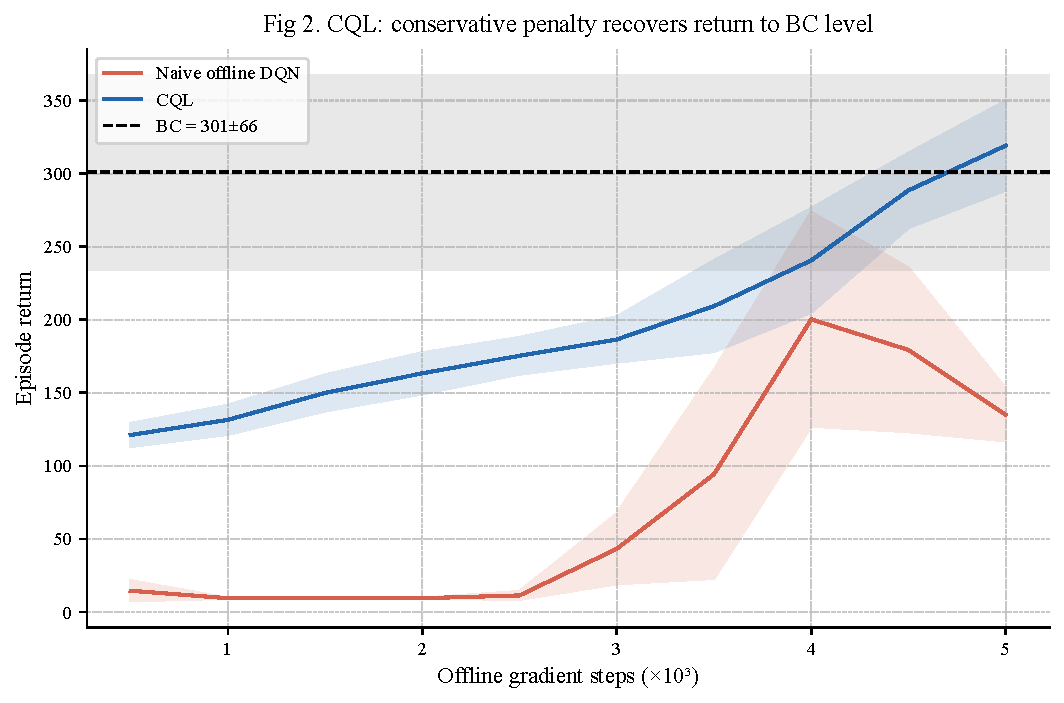
\includegraphics[width=0.88\textwidth]{fig2_cql_conservatism.pdf}
  \caption{CQL 的保守惩罚恢复回报（CartPole-v1，medium 数据集，3 个随机种子，阴影为 $\pm 1\sigma$，灰色区间为 BC 的 mean $\pm 1\sigma$）。与朴素离线 DQN 的塌缩（红色）形成对比，CQL 的回报（蓝色）随离线更新稳步上升到 BC 区间——不再塌缩。同一个框架，只多一项 $\alpha\mathcal{R}(s)$ 正则，从「塌缩」到「恢复」——惩罚把 Q 锚定在数据支持的动作上。}
  \label{fig:cql-conservatism}
\end{figure}

% ============================================================
\section*{方案二：IQL——把悲观写进动作集合}

\subsection*{直觉}

隐式 Q 学习（Implicit Q-Learning）走完全相反的路线：\textbf{永远不去评估数据外的动作}。它用一个特殊的回归目标拟合价值函数，使 $V$ 直接「跳过」$\max$——因为 $\max$ 恰恰是数据外误差的来源。

\subsection*{expectile 回归}

普通最小二乘拟合的是条件\textbf{均值}；IQL 改用 expectile 回归，用超参 $\tau\in(0,1)$ 控制拟合到条件分布的哪个分位：

\[
\boxed{L_2^\tau(u) = \bigl|\tau - \mathbf{1}\{u<0\}\bigr|\,u^2}
\]

\begin{itemize}
  \item $\tau = 0.5$ 退化为普通最小二乘（拟合均值）；
  \item $\tau > 0.5$（典型取 $0.7 \sim 0.9$）偏向拟合\textbf{上分位}——只把「数据内比较好的结果」纳入 $V$。
\end{itemize}

\textbf{翻译成人话}：在线 Q-learning 用 $\max_{a'} Q(s',\cdot)$ 回答「下一步最好能有多好」；IQL 用 expectile 回答同一句话，但\textbf{只依据数据里真实出现过的 $(s',a')$}。答案既保留了对好动作的乐观，又永远不会跑到数据之外取值。

\subsection*{价值函数与策略更新}

V 与 Q 交替回归：

\[
\boxed{V_\psi(s) \;\leftarrow\; \arg\min_V \mathbb{E}_{(s,a)\sim\mathcal{D}}\!\left[L_2^\tau\!\bigl(Q_{\bar\theta}(s,a) - V_\psi(s)\bigr)\right]}
\]

\[
\boxed{Q_\theta(s,a) \;\leftarrow\; \arg\min_Q \mathbb{E}_{(s,a,s')\sim\mathcal{D}}\!\left[\bigl(Q_\theta(s,a) - r - \gamma V_\psi(s')\bigr)^2\right]}
\]

\begin{itemize}
  \item $V$ 只从数据内动作的 $Q_{\bar\theta}$ 回归，$\tau$ 决定它偏向好动作还是均值；
  \item $Q$ 的目标里\textbf{没有 $\max$}，只有 $r + \gamma V(s')$——外推误差没有入口。
\end{itemize}

策略用 AWR 式的加权监督学习更新：只提升「数据内价值高于 $V$」的动作，

\[
\boxed{\pi_\phi \;\leftarrow\; \arg\max_\pi \mathbb{E}_{(s,a)\sim\mathcal{D}}\!\left[\exp\!\Big(\frac{1}{\lambda}\bigl(Q_\theta(s,a) - V_\psi(s)\bigr)\Big)\log\pi_\phi(a|s)\right]}
\]

其中 $\lambda>0$ 是行为克隆与价值提升之间的\textbf{权衡温度}：$\lambda\to\infty$ 时权重趋于 1，退化为纯 BC；$\lambda\to 0$ 时权重集中于优势最大的动作，退化为贪心 Q 最大化。

\begin{figure}[!htbp]
  \centering
  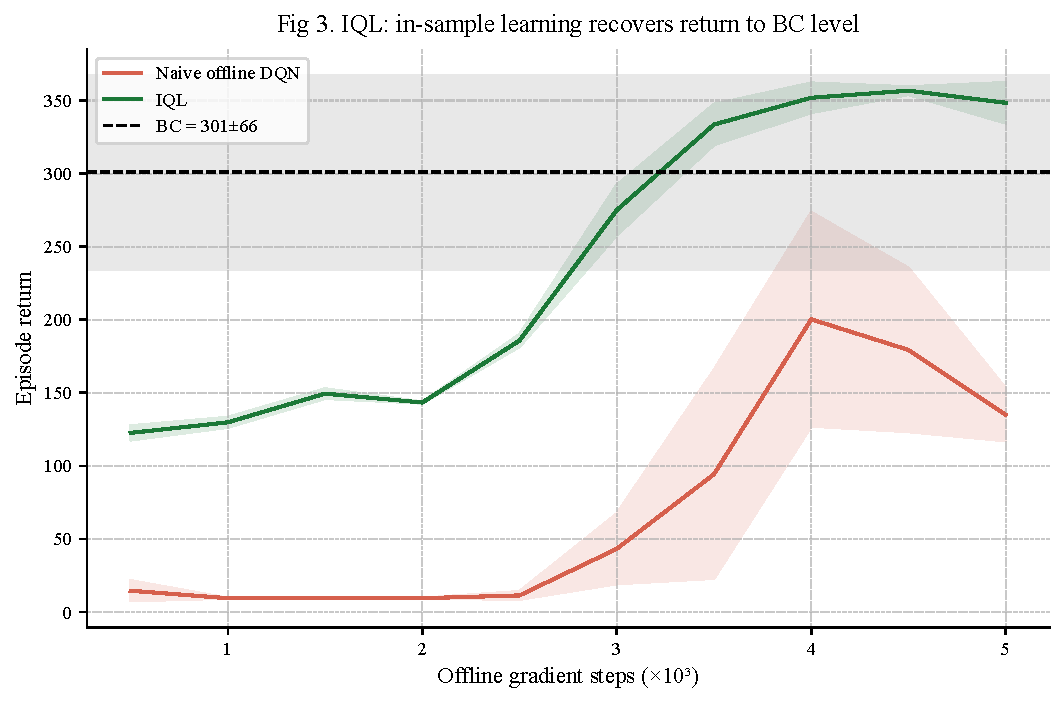
\includegraphics[width=0.88\textwidth]{fig3_iql_insample.pdf}
  \caption{IQL 的 in-sample 学习恢复回报（CartPole-v1，medium 数据集，3 个随机种子，阴影为 $\pm 1\sigma$，灰色区间为 BC 的 mean $\pm 1\sigma$）。与朴素离线 DQN 的塌缩（红色）形成对比，IQL 的回报（绿色）随离线更新稳步上升到 BC 区间——不再塌缩。它从不查询数据外动作，外推误差根本不会进入自举目标。同一个病，换一种「不问」的药，同样治好了。}
  \label{fig:iql-insample}
\end{figure}

% ============================================================
\section*{两种悲观的分工：CQL vs IQL}

\subsection*{一个病，两种药}

\begin{center}
\begin{tabular}{c|c|c}
 & \textbf{CQL} & \textbf{IQL} \\
\hline
悲观的对象 & 价值函数（压 OOD 的 Q） & 动作集合（不评估 OOD） \\
是否查询数据外动作 & 是，但压低其价值 & 从不 \\
自举目标 & 带惩罚的 $\max$ & $r + \gamma V$（无 $\max$） \\
关键超参 & 保守强度 $\alpha$ & 期望分位 $\tau$、温度 $\lambda$ \\
核心算子 & $\log\sum_a\exp Q$ & expectile 回归 $L_2^\tau$ \\
\end{tabular}
\end{center}

\textbf{设计哲学的差别}：CQL 回答的是「\underline{数据外动作值多少}」——它强行给出答案，但给的是负面的（保守的）；IQL 回答的是「\underline{不回答数据外动作}」——它修改问题本身，让 $\max$ 从算法里消失。前者是给说谎者设罚则，后者是干脆不问不知道的人。

\textbf{在实际中}：IQL 的 AWR 式策略提取往往更贴合「离线训练 + 在线微调」的流程；CQL 若要在线微调，需显式退火保守强度 $\alpha$——惩罚项不会随训练自己消失，过强的保守性会阻碍继续提升。IQL 实现也更简单、对离散/连续动作同样自然——它不需要估计行为策略的动作密度（连续情形下 CQL 要额外采样 $a\sim\hat\mu$），只需直接用数据里的 $(s,a)$ 对。两者在 D4RL 基准上各有擅长，但都能把回报稳定恢复到 BC 及格线水平——这正是本章图 2、图 3 想传达的：两条路殊途同归。

% ============================================================
\section*{本章在 RL 体系中的位置}

\begin{enumerate}
  \item \textbf{值函数路线} $\to$ DQN（在线 $\max$）$\to$ 双 Q / 目标网络（缓解过估计）；
  \item \textbf{Off-policy 路线} $\to$ \underline{SAC}（上一章：replay buffer 反复利用）——离线 RL 就是「拔掉环境插头，把 buffer 固化成整个数据集」；
  \item \underline{离线强化学习}（本章：不能交互，只读固定数据集 $\to$ 分布漂移 $\to$ CQL 压 OOD 价值 / IQL 不问 OOD）；
  \item \textbf{下游} $\to$ 保守思想的延伸（model-based 离线方法）；决策 Transformer（第 11 章）则换一套序列建模的世界观重答本章的问题。
\end{enumerate}

离线 RL 是 RL 走向工业落地的关键一环：真实系统的数据贵、风险高，很多时候只有历史数据可用。本章的两套方案代表了领域内两种主流的「悲观」设计——约束价值，或约束动作——它们共同确立了离线学习的及格线思维：不塌缩（恢复到 BC 水平）比聪明（追最优）更重要。

\subsection*{参考资料}

\begin{enumerate}
  \item Kumar et al.\ (2020). Conservative Q-Learning for Offline Reinforcement Learning. \textit{NeurIPS}.
  \item Kostrikov, Nair \& Levine (2021). Offline Reinforcement Learning with Implicit Q-Learning. \textit{NeurIPS}.
  \item Fujimoto, Meger \& Precup (2019). Off-Policy Deep Reinforcement Learning without Exploration. \textit{ICML}.
  \item Levine et al.\ (2020). Offline Reinforcement Learning: Tutorial, Review, and Perspectives on Practical Applications. \textit{arXiv:2005.01643}.
  \item Pomerleau (1991). Efficient Training of Artificial Neural Networks for Autonomous Navigation. \textit{Neural Computation}.
  \item Sutton \& Barto (2018). \textit{Reinforcement Learning: An Introduction} (2nd ed.). Chapter 13.
\end{enumerate}

\end{document}
